\section{Results} \label{sec:results}

\begin{itemize}
\item There isn't a whole lot of flexibility for SFR=0 galaxies predicted by
simulations and they do not agree well with observations \ref{sec:res}. 
\end{itemize}

\begin{figure}
\begin{center}
    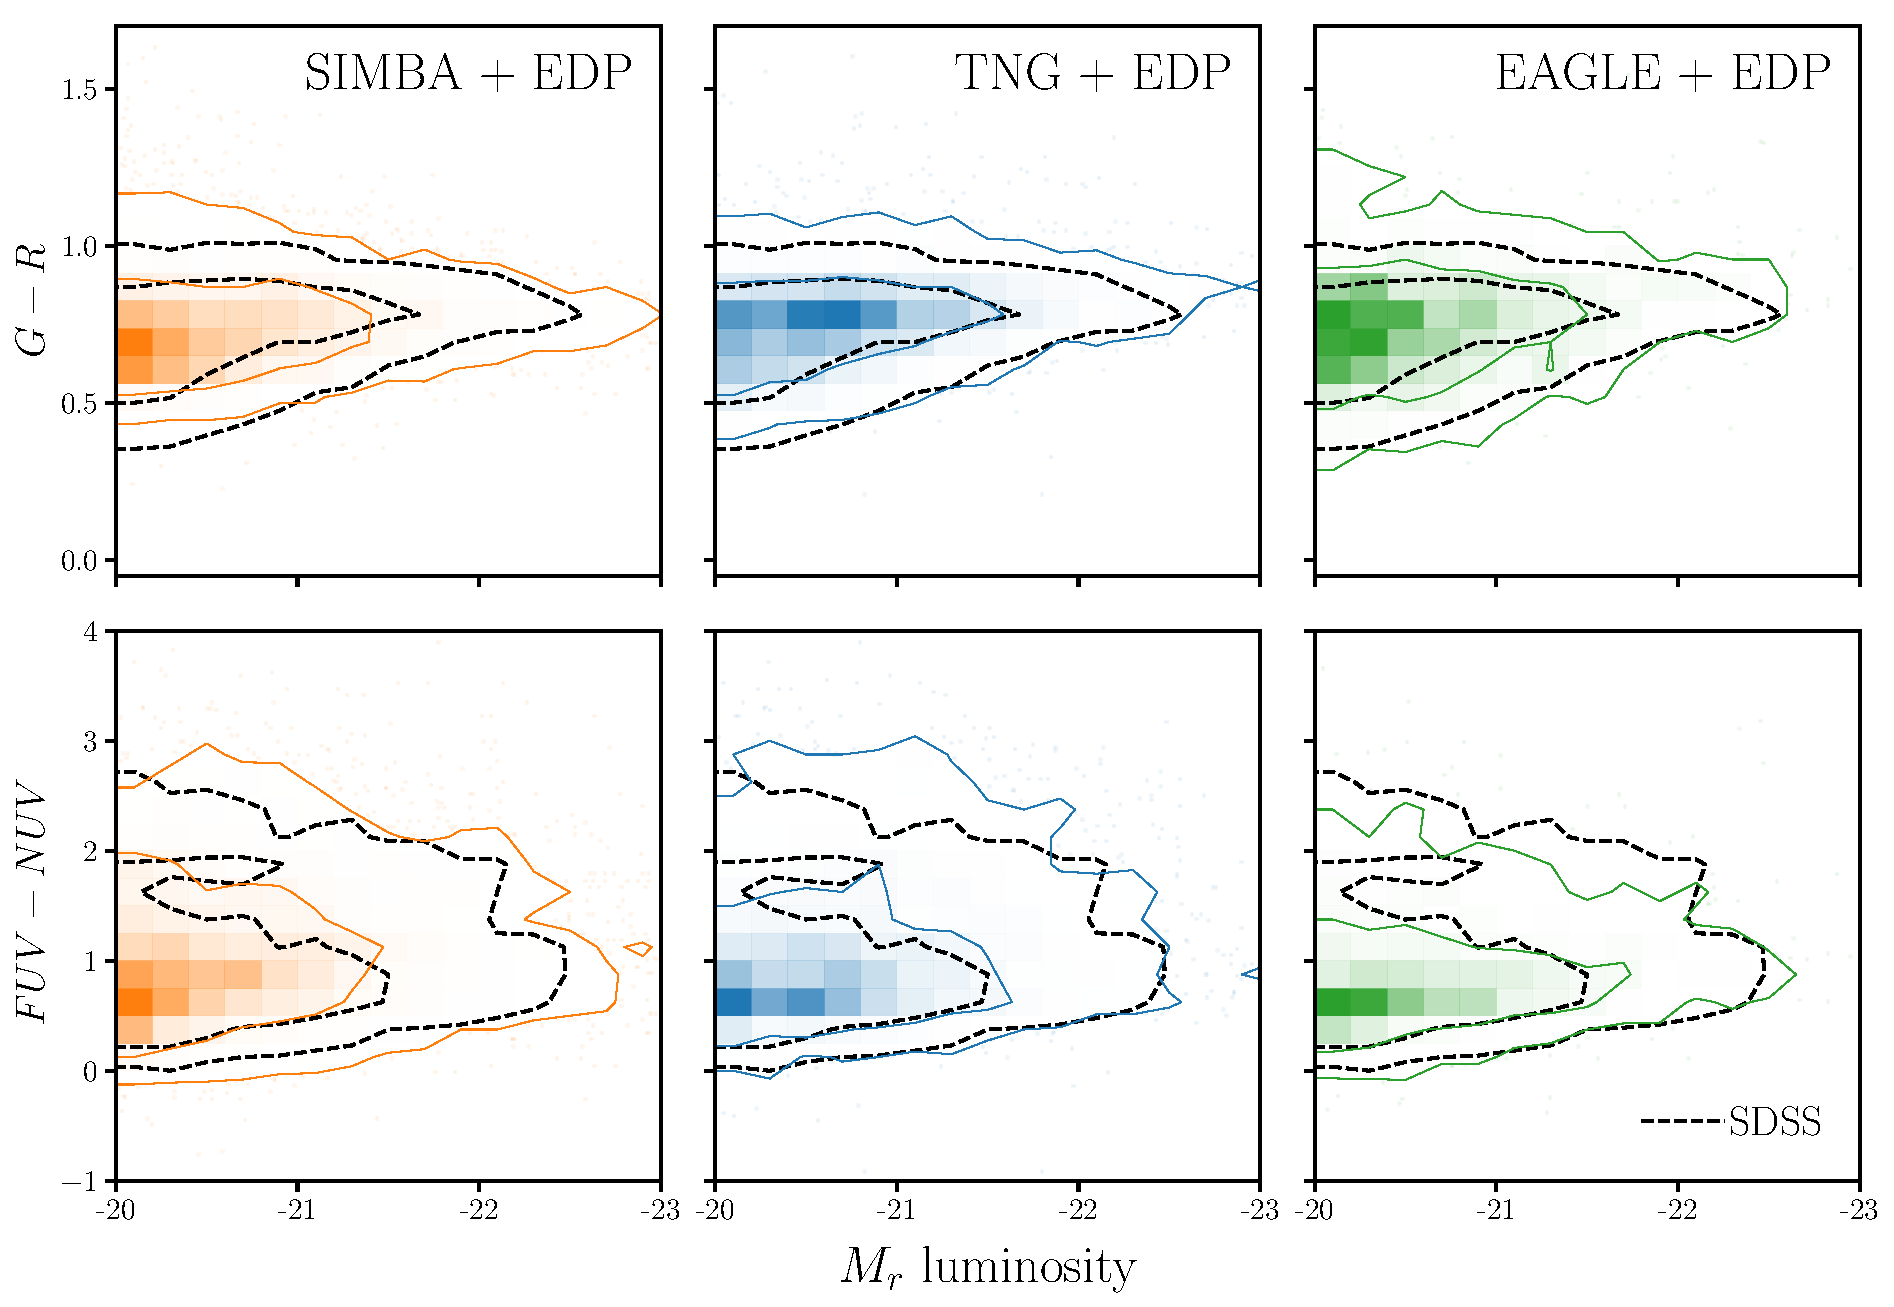
\includegraphics[width=\textwidth]{figs/abc_observables.pdf}
    \caption{Comparison of the observables predicted by the simulations with
    the posterior DEM.}
\label{fig:dem}
\end{center}
\end{figure}

\begin{figure}
\begin{center}
    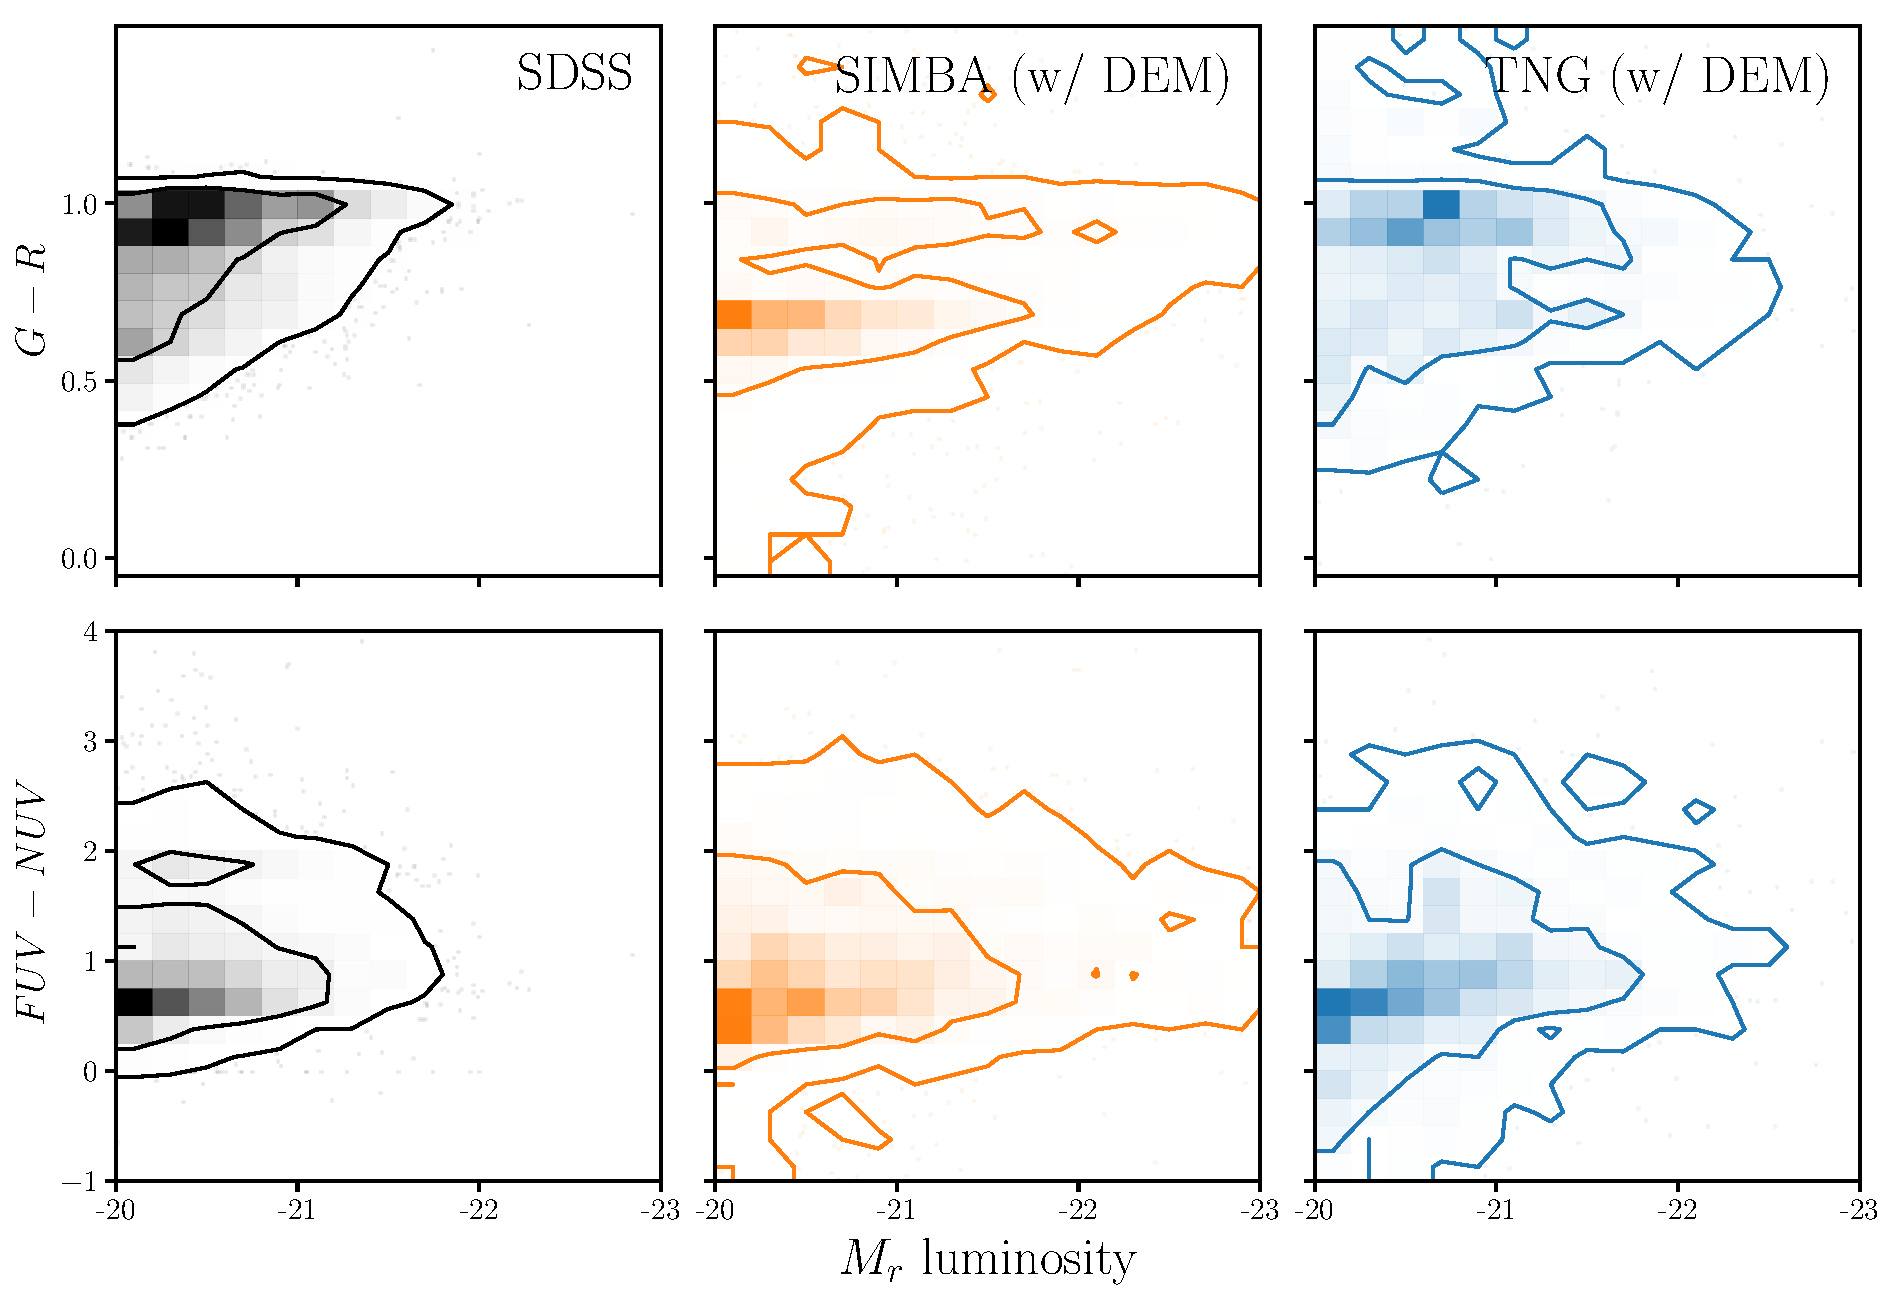
\includegraphics[width=\textwidth]{figs/abc_tnorm_observables.pdf}
    \caption{Comparison of the observables predicted by the simulations with
    the posterior DEM.}
\label{fig:dem}
\end{center}
\end{figure}


\begin{figure}
\begin{center}
    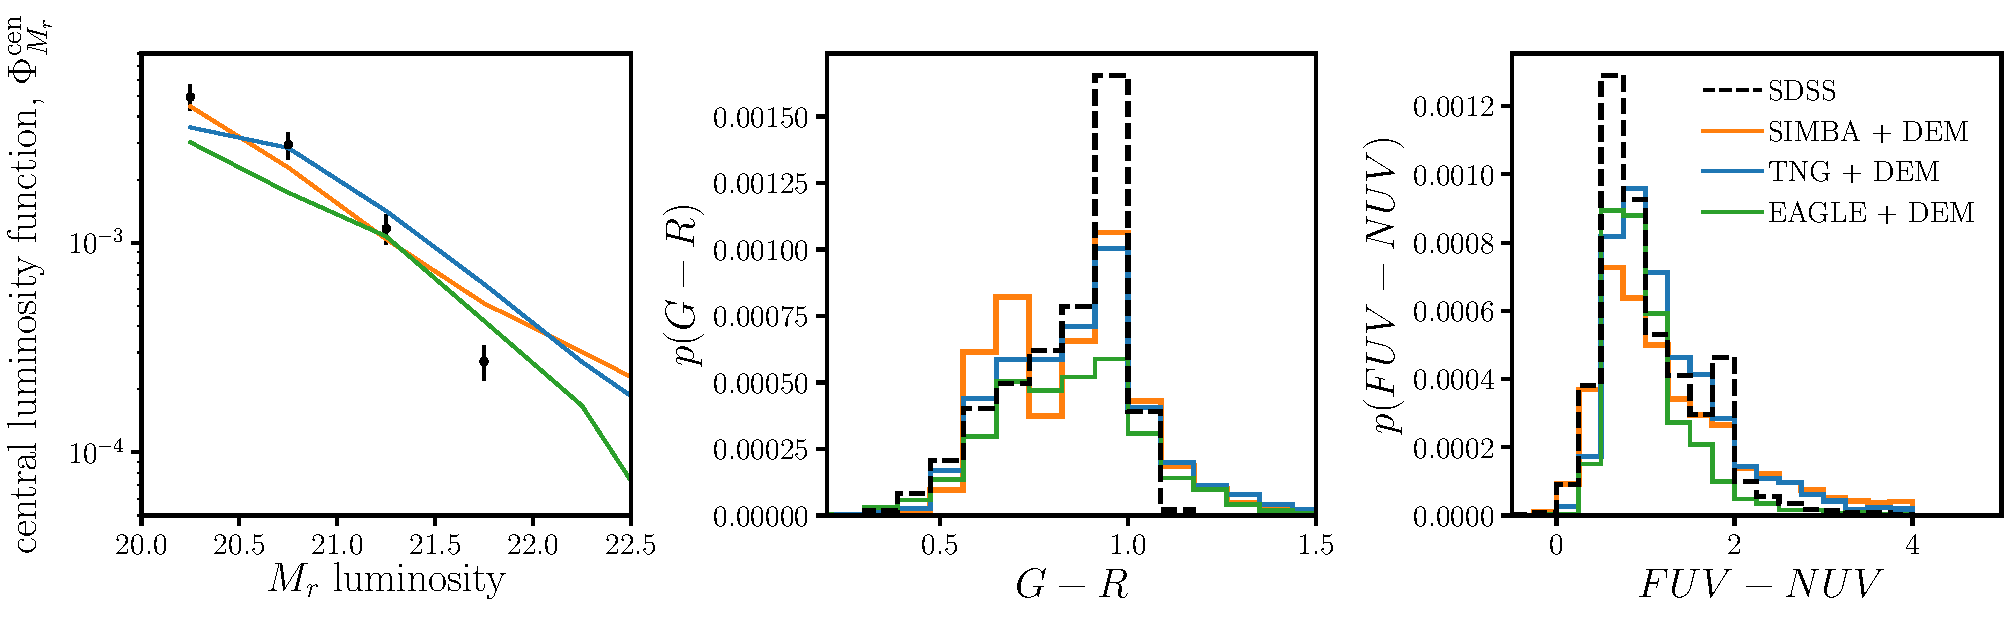
\includegraphics[width=\textwidth]{figs/abc_observables_1d.pdf}
    \caption{Comparison of the observables predicted by the simulations with
    the posterior DEM.}
\label{fig:dem}
\end{center}
\end{figure}

\begin{figure}
\begin{center}
    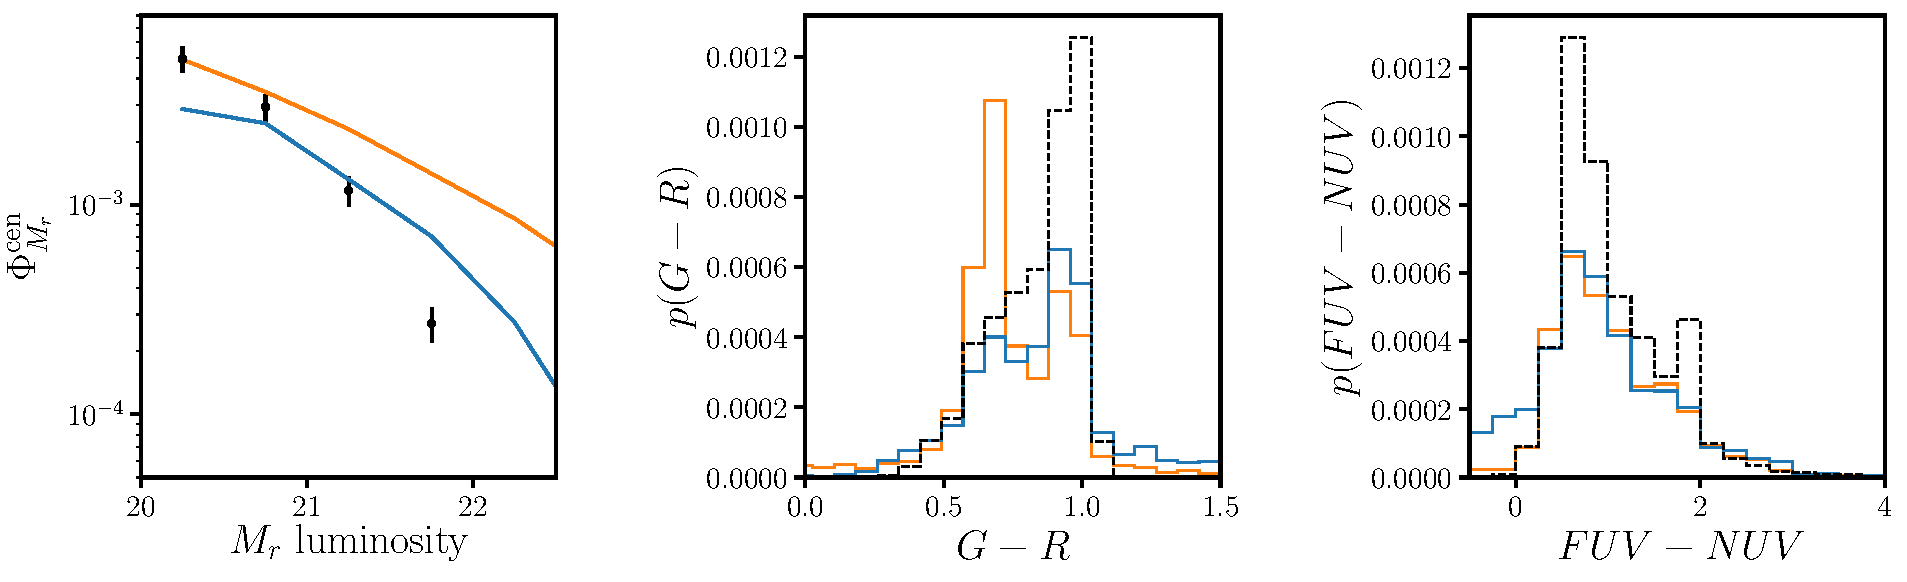
\includegraphics[width=\textwidth]{figs/abc_tnorm_observables_1d.pdf}
    \caption{Comparison of the observables predicted by the simulations with
    the posterior DEM.}
\label{fig:dem}
\end{center}
\end{figure}
